
Given pattern \texttt{((n ...) ...)} (\texttt{n} is shorthand for \texttt{number}) and term \texttt{((1 2 3)())}, the matching algorithm should return a \texttt{Match} instance pattern-variable assignment \texttt{number = ((1 2 3) ())}. The diagram below shows how using the \texttt{increasedepth} and \texttt{decreasedepth} methods provided by `Match` facilitate the matching. 

\begin{figure}[h]
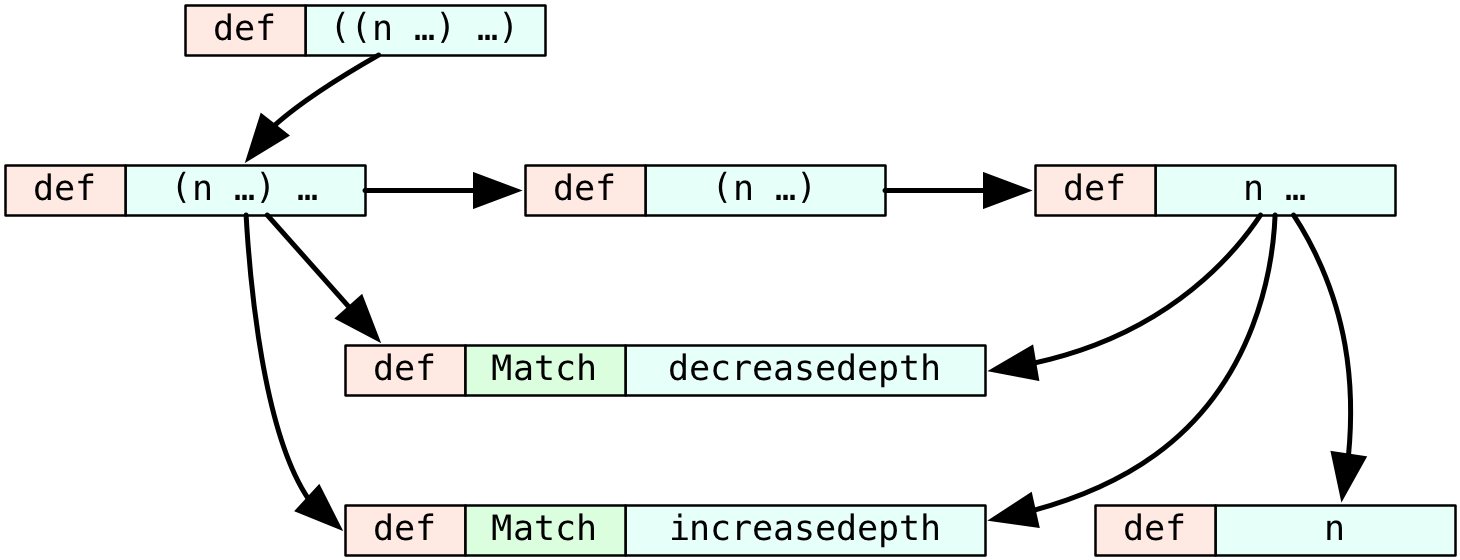
\includegraphics[scale=0.25]{ellipsis-example-callgraph.png}
\caption{Callgraph for function matching pattern \texttt{((n ...) ...)}}
\label{ellipsis-example-callgraph}
\end{figure}

Callgraph for function matching pattern \texttt{((n ...) ...)} can be seen in Figure \ref{ellipsis-example-callgraph}. Code generation algorithm generates five matching functions for this pattern:

\begin{enumerate}
\item function for pattern \texttt{((n ...) ...)}
\item function for pattern \texttt{(n ...) ...}
\item function for pattern \texttt{(n ...) }
\item function for pattern \texttt{n ... }
\item function for pattern \texttt{n}
\end{enumerate}

Figure \ref{ellipsis-example-fig-a} show state of \texttt{Match} object before beginning to match a term (red nodes) against a pattern (blue nodes). Outlined pattern nodes represent the current sub-pattern being matched; and since matching hasn't begun yet the entire pattern is outlined. The same applies to the term. Initially, \texttt{Binding} instance assigned to pattern variable \texttt{n} in \texttt{Match} instance has an empty stack.

Figure \ref{ellipsis-example-fig-b} shows state of \texttt{Match} object after entering generated function for \textit{outer} ellipsis and calling \texttt{increasedepth("n")} method. This pushes empty \texttt{Sequence} onto the stack.


Figure \ref{ellipsis-example-fig-c} shows state of \texttt{Match} object after entering generated function for \textit{inner} ellipsis and calling \texttt{increasedepth("n")} method. This pushes empty \texttt{Sequence} onto the stack. The term now contains two \texttt{Sequence} instances.

Figure \ref{ellipsis-example-fig-d} shows matching of term \texttt{Integer(1)}. Need to call \texttt{addtobinding} method with \texttt{"n"} and \texttt{Integer(1)} as arguments. Since topmost term on the stack is \texttt{Sequence}, \texttt{Integer(1)} is appended to it.

Figures \ref{ellipsis-example-fig-e} and \ref{ellipsis-example-fig-f} call \texttt{addtobinding} with \texttt{Float(2.01)} and \texttt{Integer(3)}. Both terms are appended to the topmost \texttt{Sequence} on the stack.

All terms in \texttt{Sequence} have been consumed. Figure \ref{ellipsis-example-fig-g} shows state of the match object after calling \texttt{decreasedepth("n")}. Since the stack contains to \texttt{Sequence} instances, topmost one is removed from stack and appended to the first \texttt{Sequence}. Function for \textit{inner} ellipsis is exited.

Now, the remaining empty term sequence has to be matched, as seen in Figure \ref{ellipsis-example-fig-h}.

Figure \ref{ellipsis-example-fig-i} shows state of \texttt{Match} object after entering the generated function for \textit{inner} ellipsis. Empty \texttt{Sequence} instance is pushed onto the stack.

Since the term sequence is empty, function for \texttt{Number} pattern cannot be called. Figure \ref{ellipsis-example-fig-j} shows the state of the \texttt{Match} object after calling \texttt{decreasedepth("n")}. Since the stack contains two \texttt{Sequence} instances, the topmost one is popped from the stack and appended to previous \texttt{Sequence}. Function for \textit{inner} ellipsis is exited.

Finally, there are no more terms to match in outermost sequence and \texttt{decreasedepth("n")} has to be called, as shown in Figure \ref{ellipsis-example-fig-k}. Since the stack only contains a single term, no action is performed. The \texttt{Match} contains assignment \texttt{n = ((1 2 3)())}, as expected.

\begin{figure}[H]
\caption{Lifetime of \texttt{Match} object}
%\begin{adjustwidth}{-1cm}{1cm}
\fbox{
	\begin{subfigure}{0.5\linewidth}
		\raisebox{5mm}{
			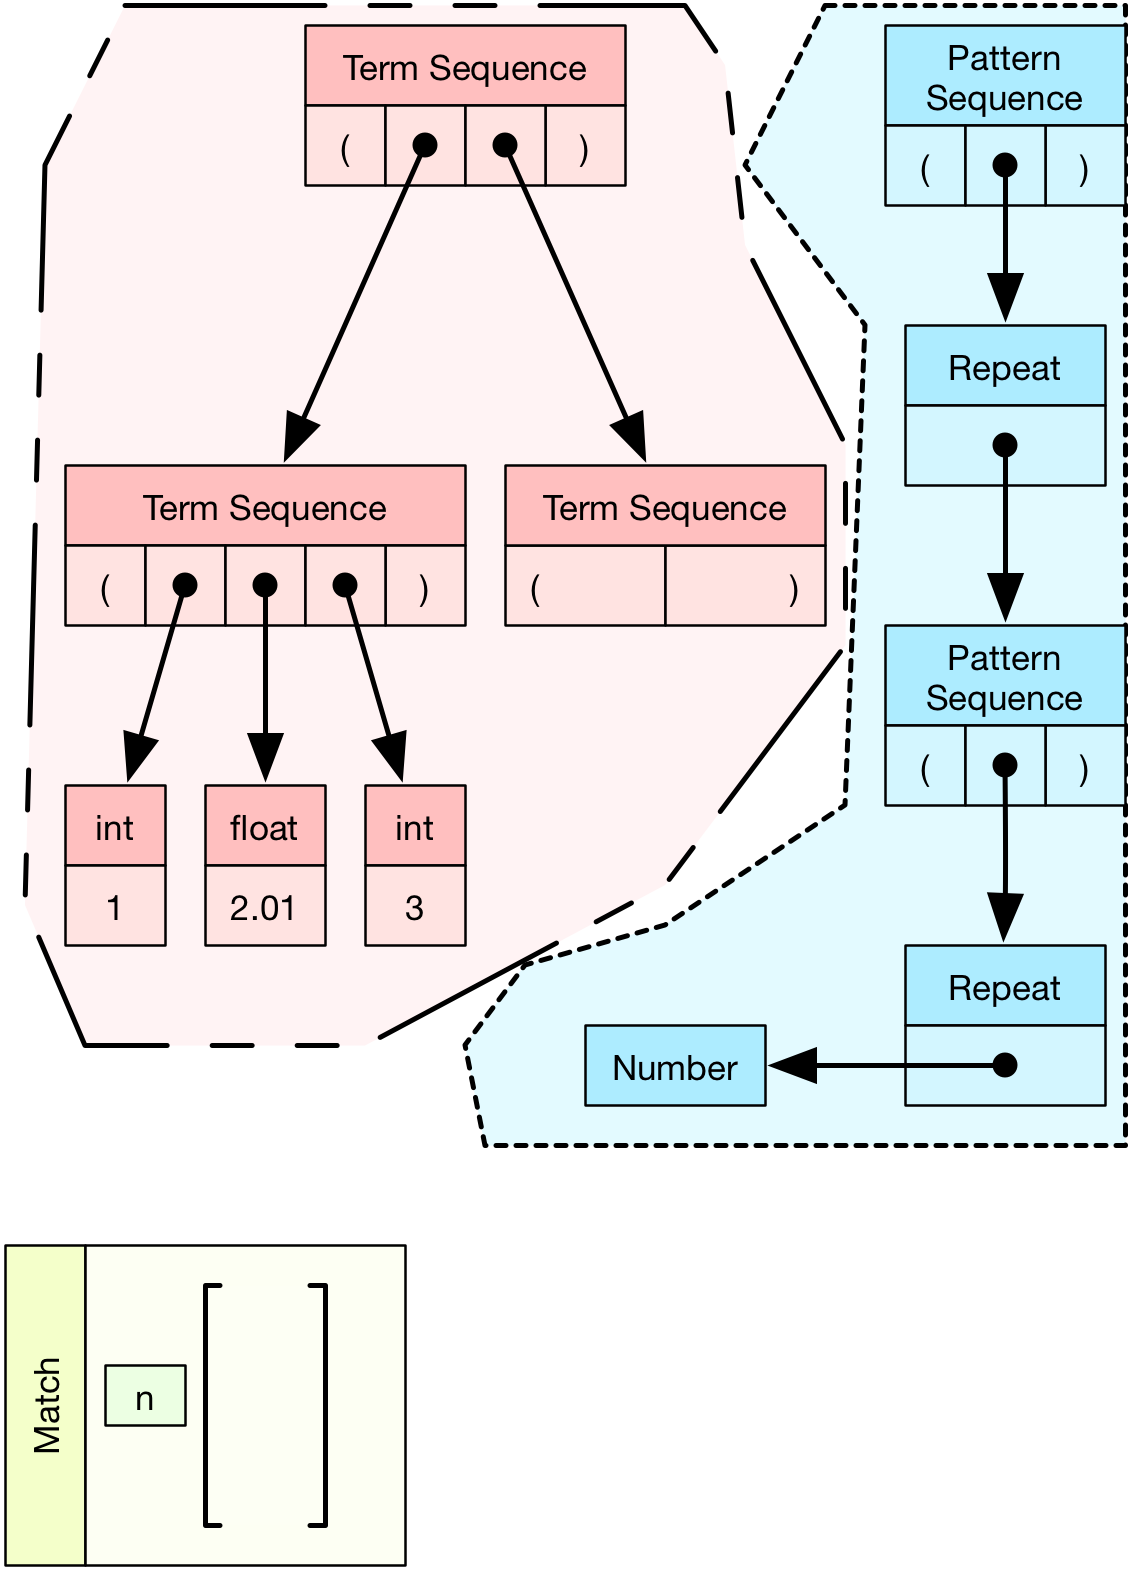
\includegraphics[scale=0.152]{ellipsis-example-fig-a.png}
		}
		\caption{Before matching the pattern.}
		\label{ellipsis-example-fig-a}
	\end{subfigure}
	\begin{subfigure}{0.5\linewidth}
		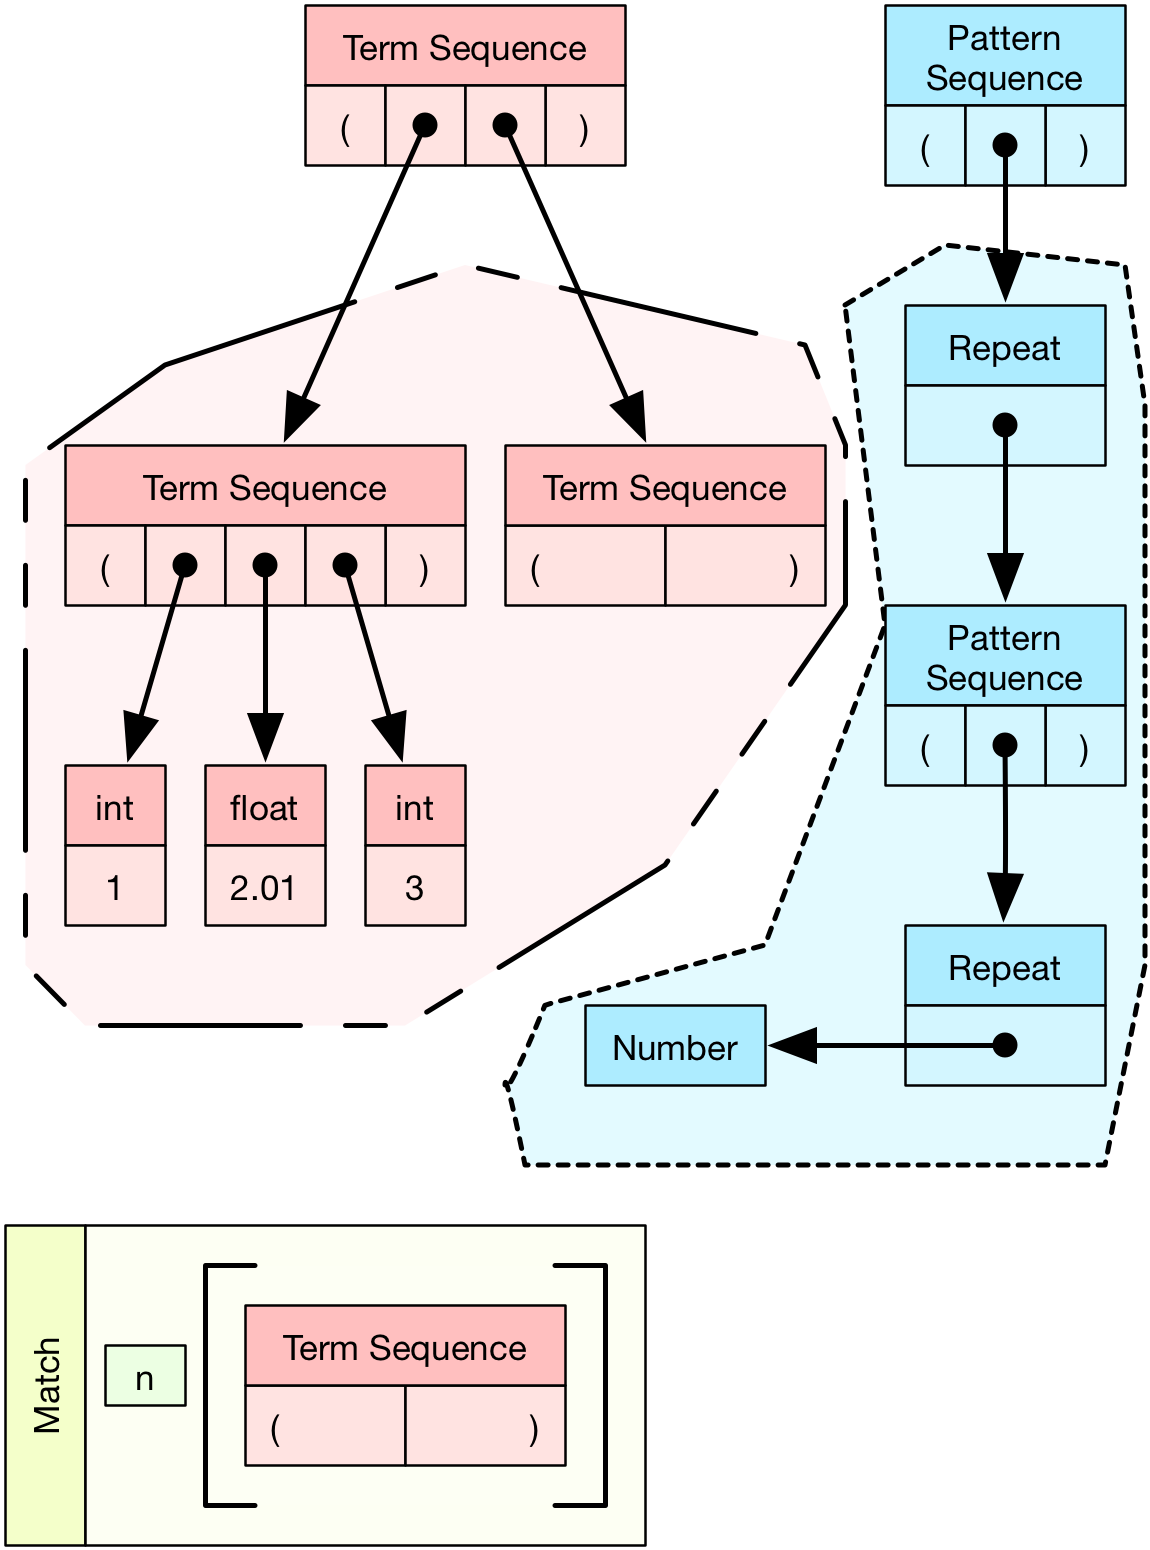
\includegraphics[scale=0.152]{ellipsis-example-fig-b.png}
		\caption{Enter outer ellipsis and \texttt{increasedepth("n")}.}
		\label{ellipsis-example-fig-b}
	\end{subfigure}
}

\fbox{
	\begin{subfigure}{0.5\linewidth}
		\raisebox{19mm}{
			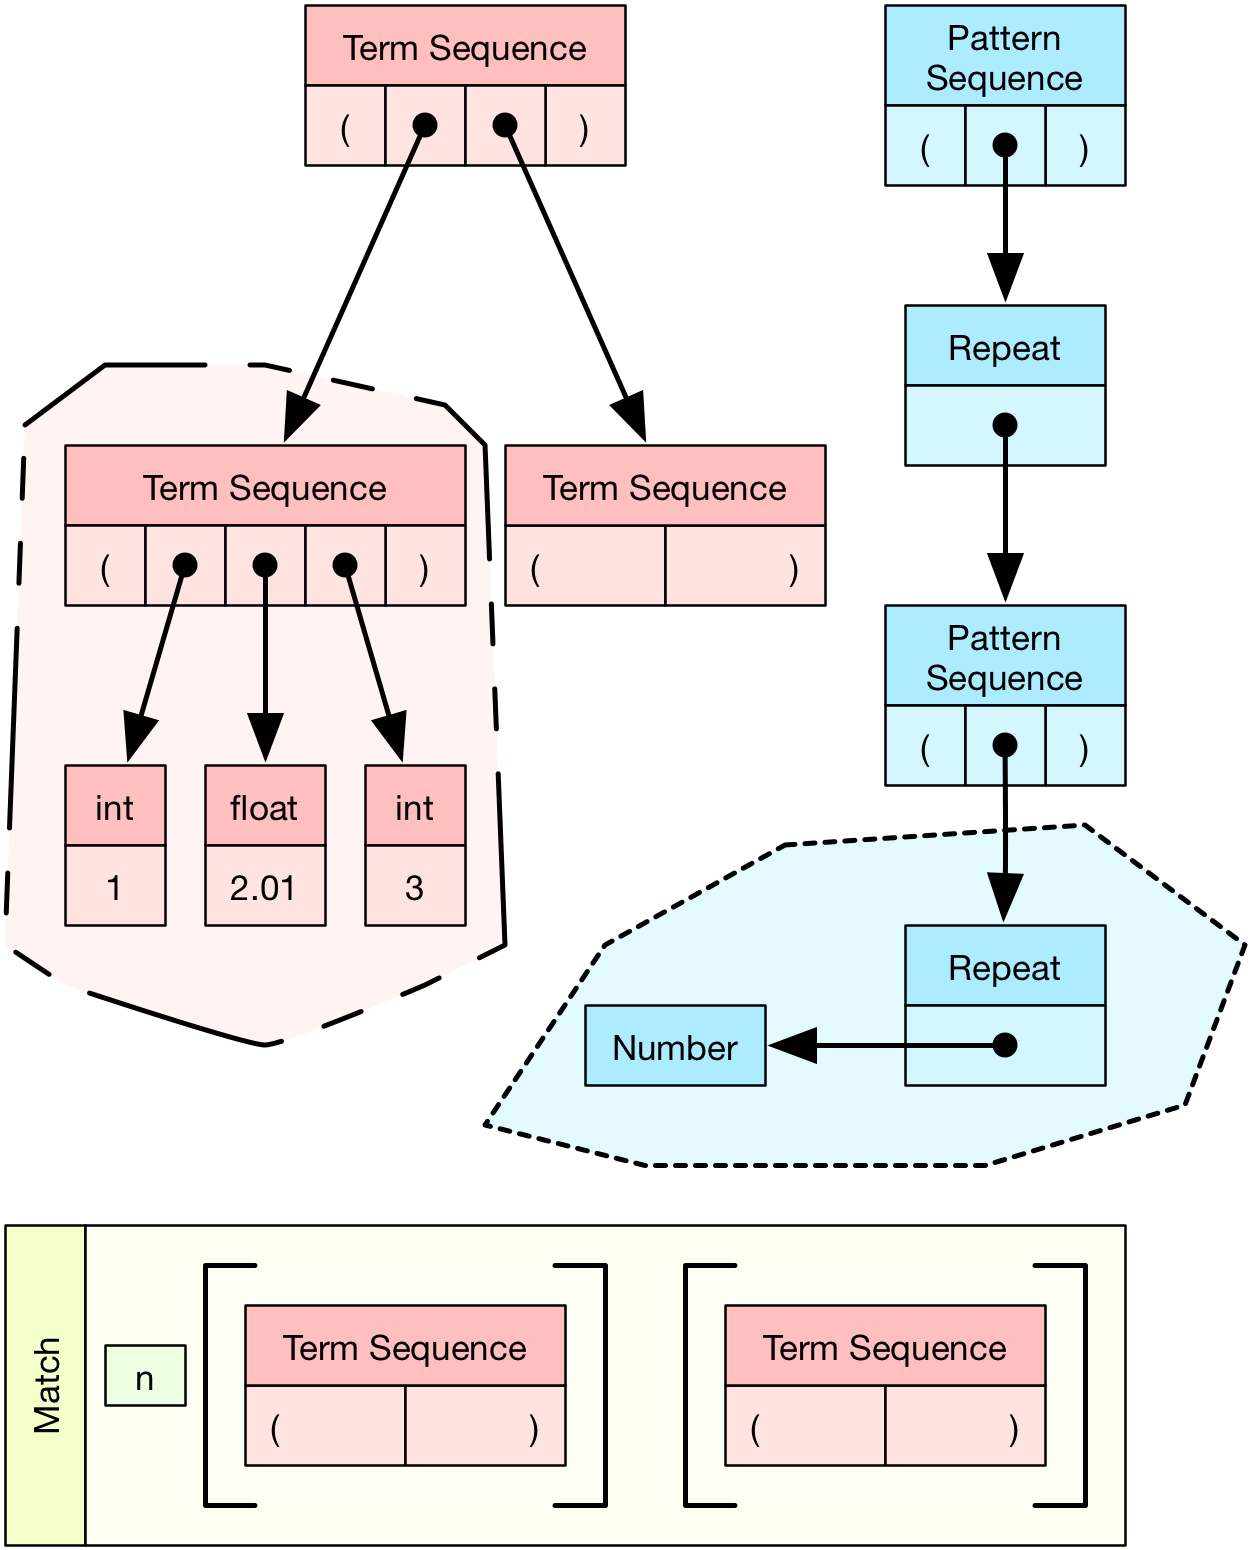
\includegraphics[scale=0.152]{ellipsis-example-fig-c.png}
		}
		\caption{Enter inner ellipsis and \texttt{increasedepth("n")}.}
		\label{ellipsis-example-fig-c}
	\end{subfigure}
	\begin{subfigure}{0.5\linewidth}
		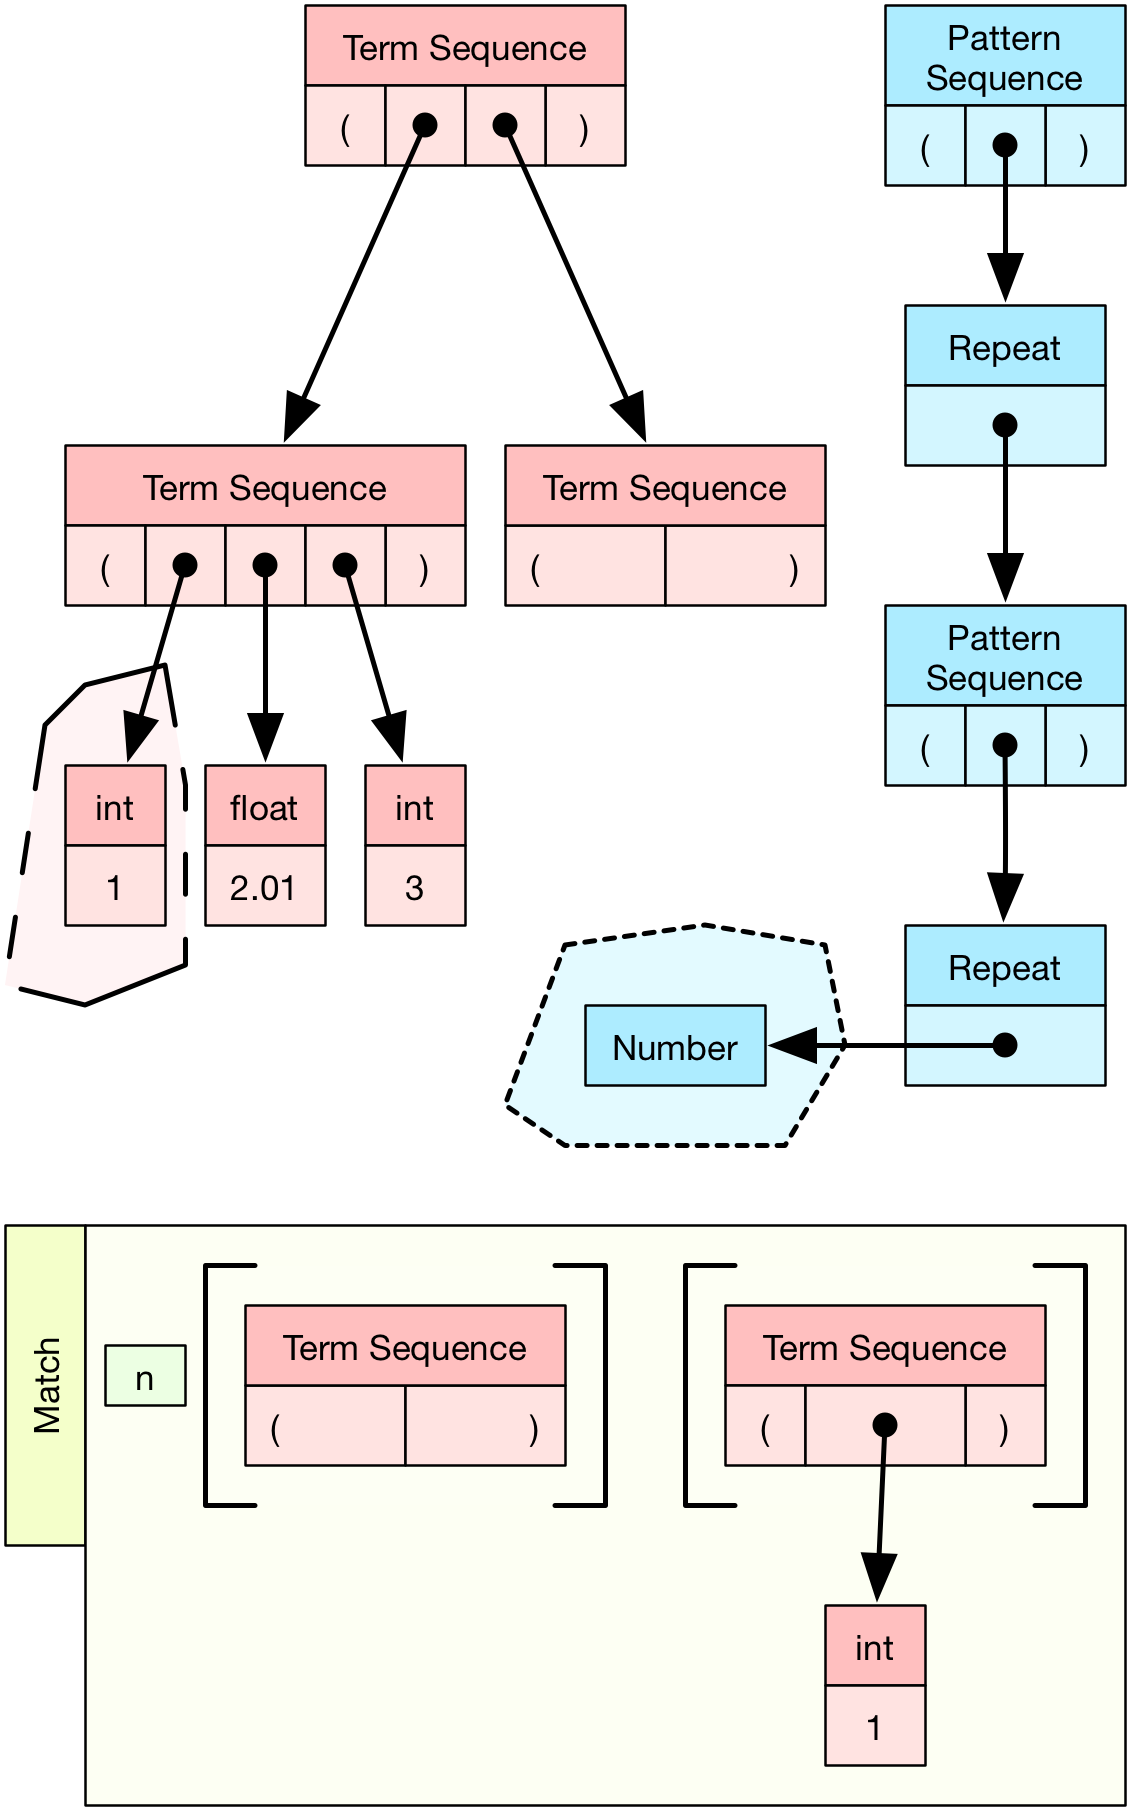
\includegraphics[scale=0.152]{ellipsis-example-fig-d.png}
		\caption{\texttt{addtobinding("n", Integer(1))}}
		\label{ellipsis-example-fig-d}
	\end{subfigure}
}

%\end{adjustwidth}
\end{figure}

\begin{figure}[H]\ContinuedFloat
\fbox{
	\begin{subfigure}{0.5\linewidth}
		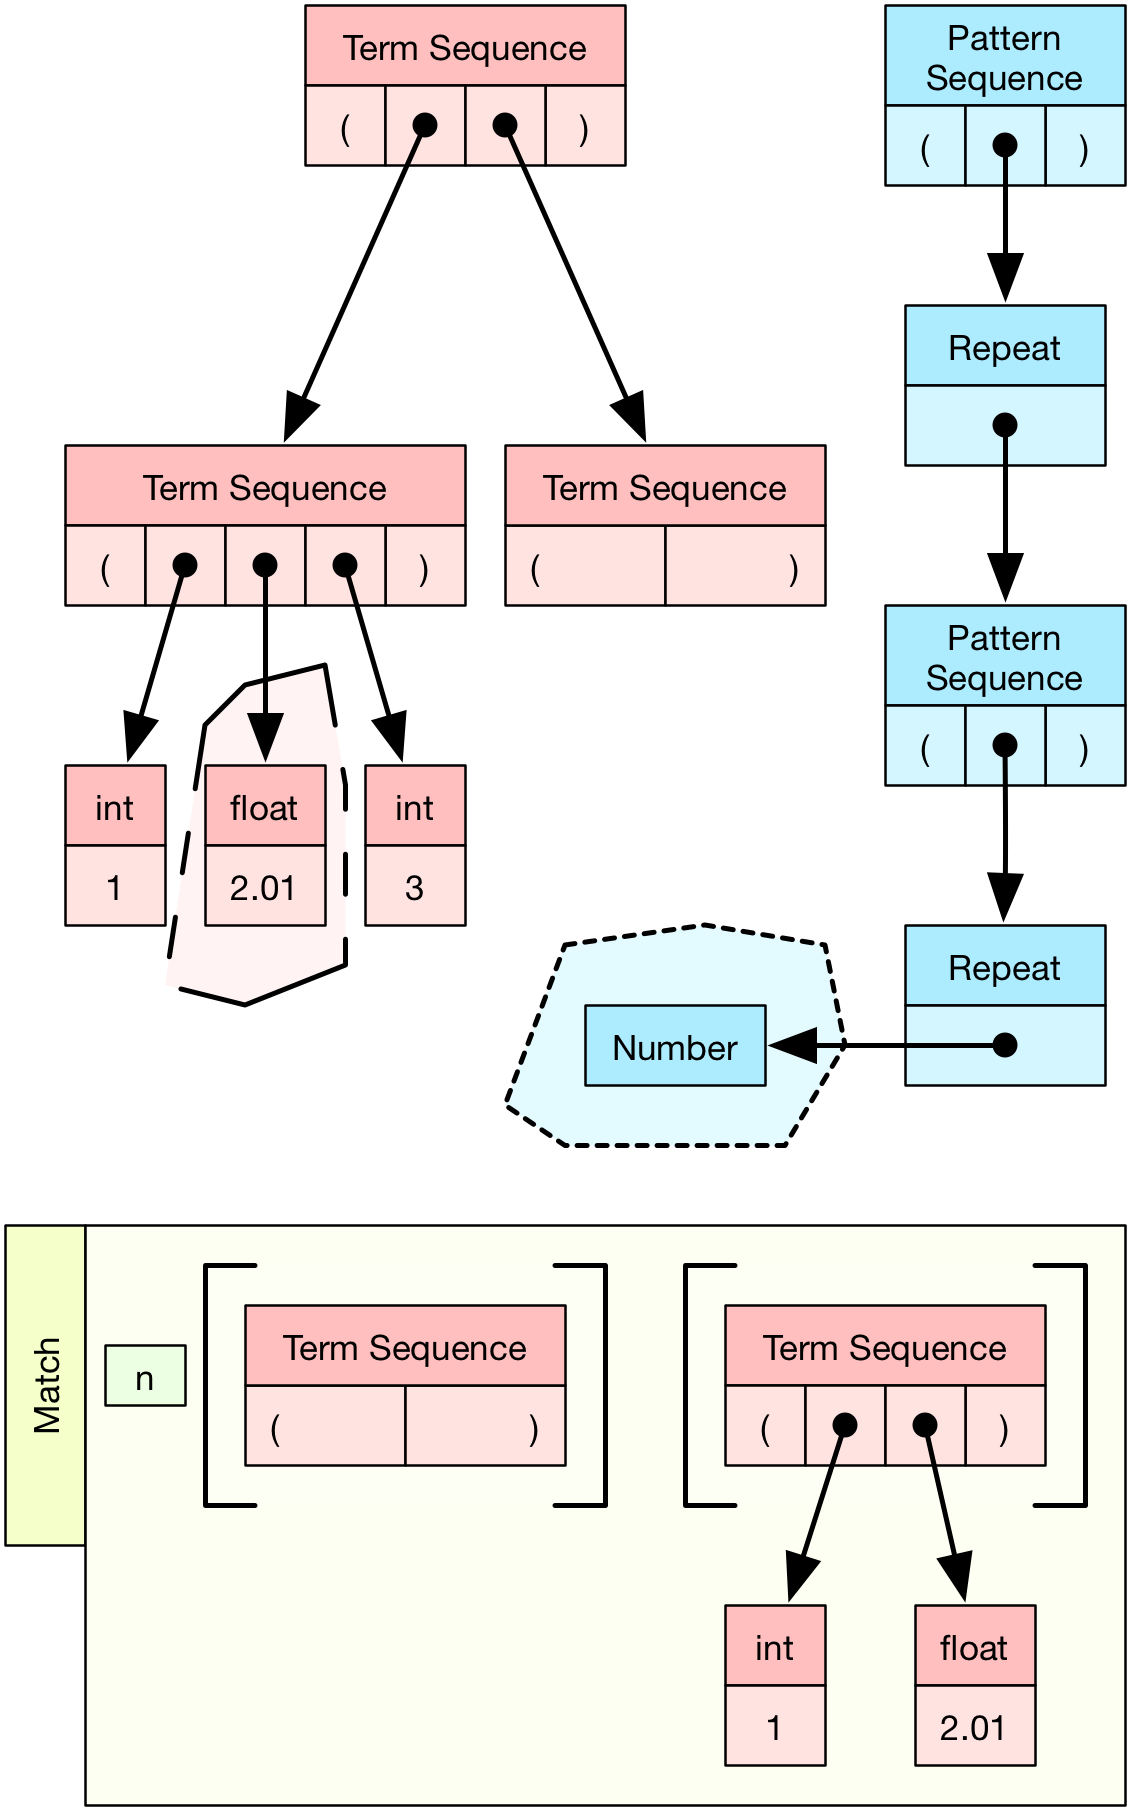
\includegraphics[scale=0.152]{ellipsis-example-fig-e.png}
		\caption{\texttt{addtobinding("n", Float(2.01))}}
		\label{ellipsis-example-fig-e}
	\end{subfigure}
	\begin{subfigure}{0.5\linewidth}
		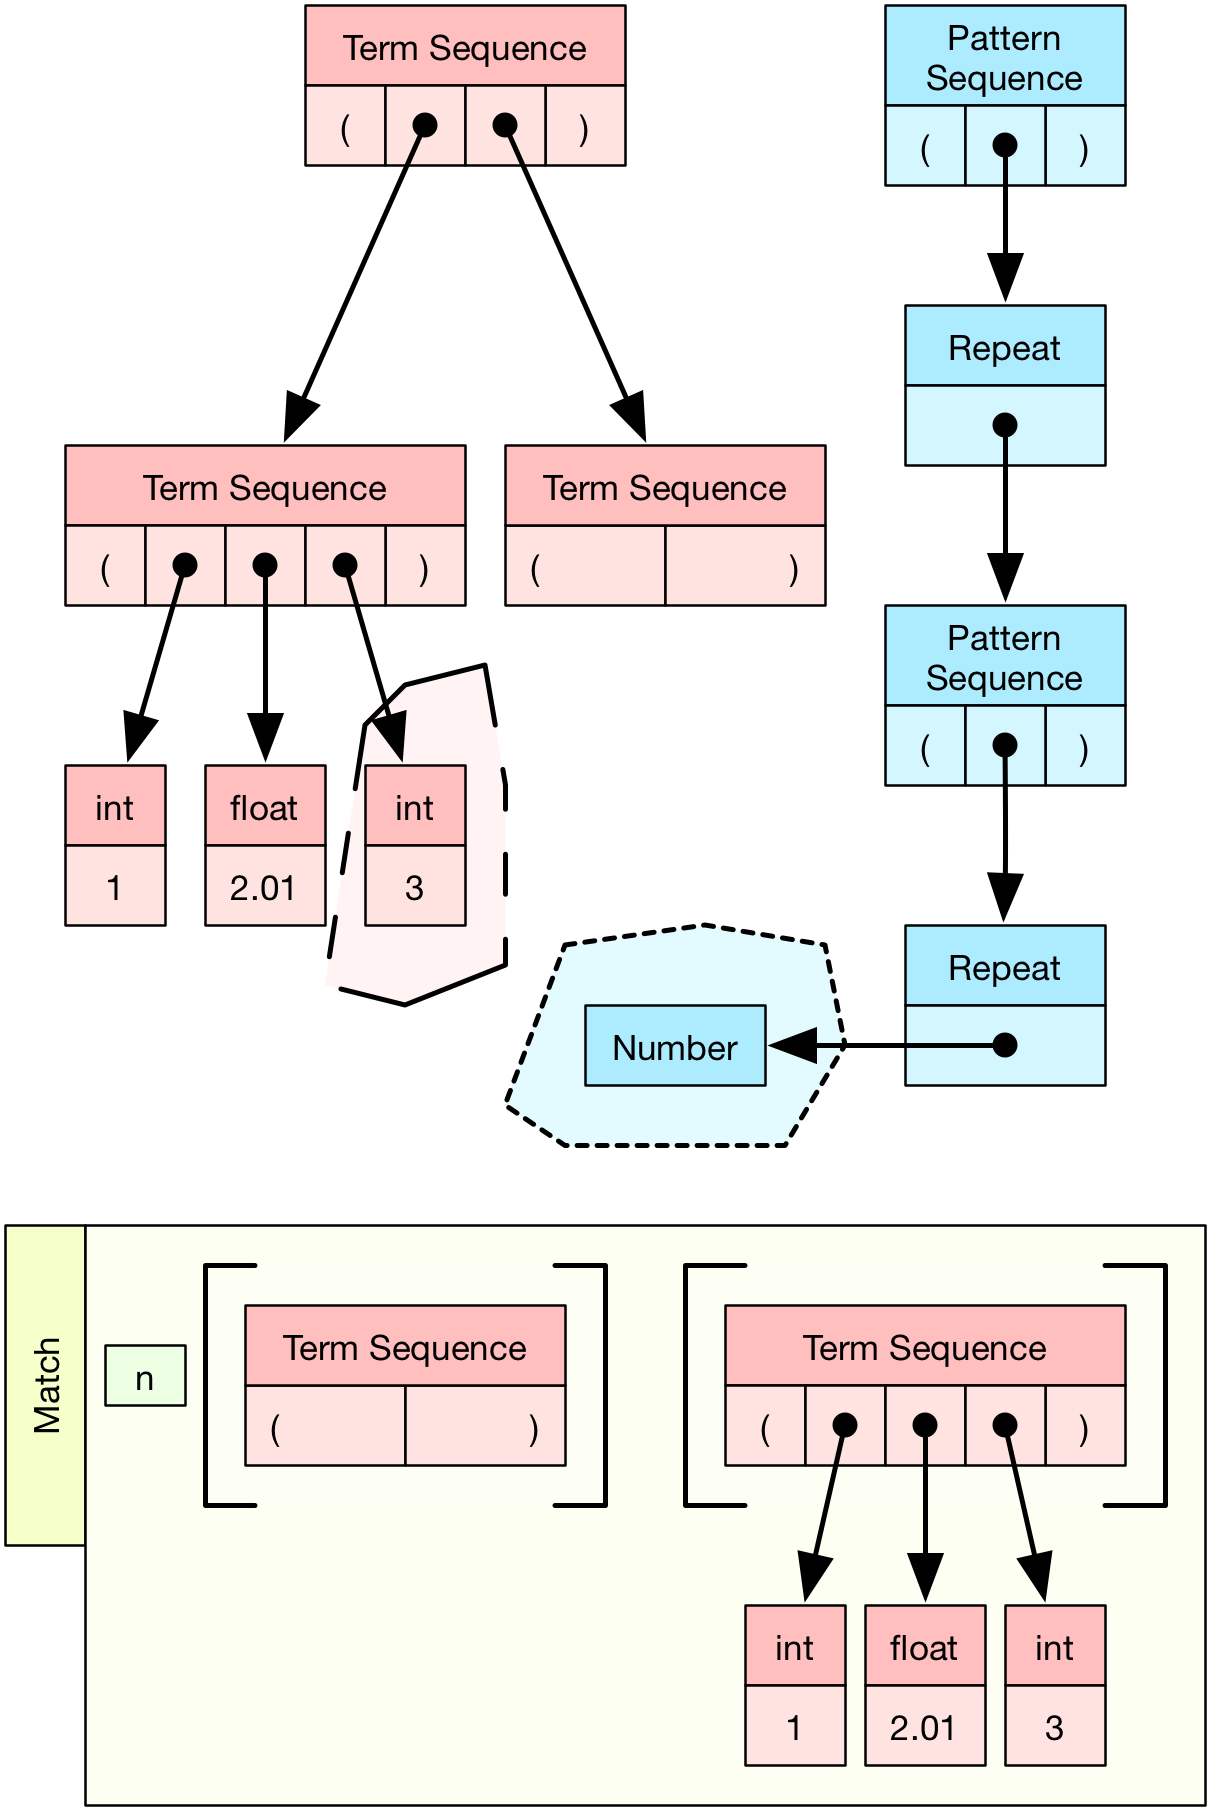
\includegraphics[scale=0.152]{ellipsis-example-fig-f.png}
		\caption{\texttt{addtobinding("n", Integer(3))}}
		\label{ellipsis-example-fig-f}
	\end{subfigure}
}
\fbox{
\begin{subfigure}{0.5\linewidth}
	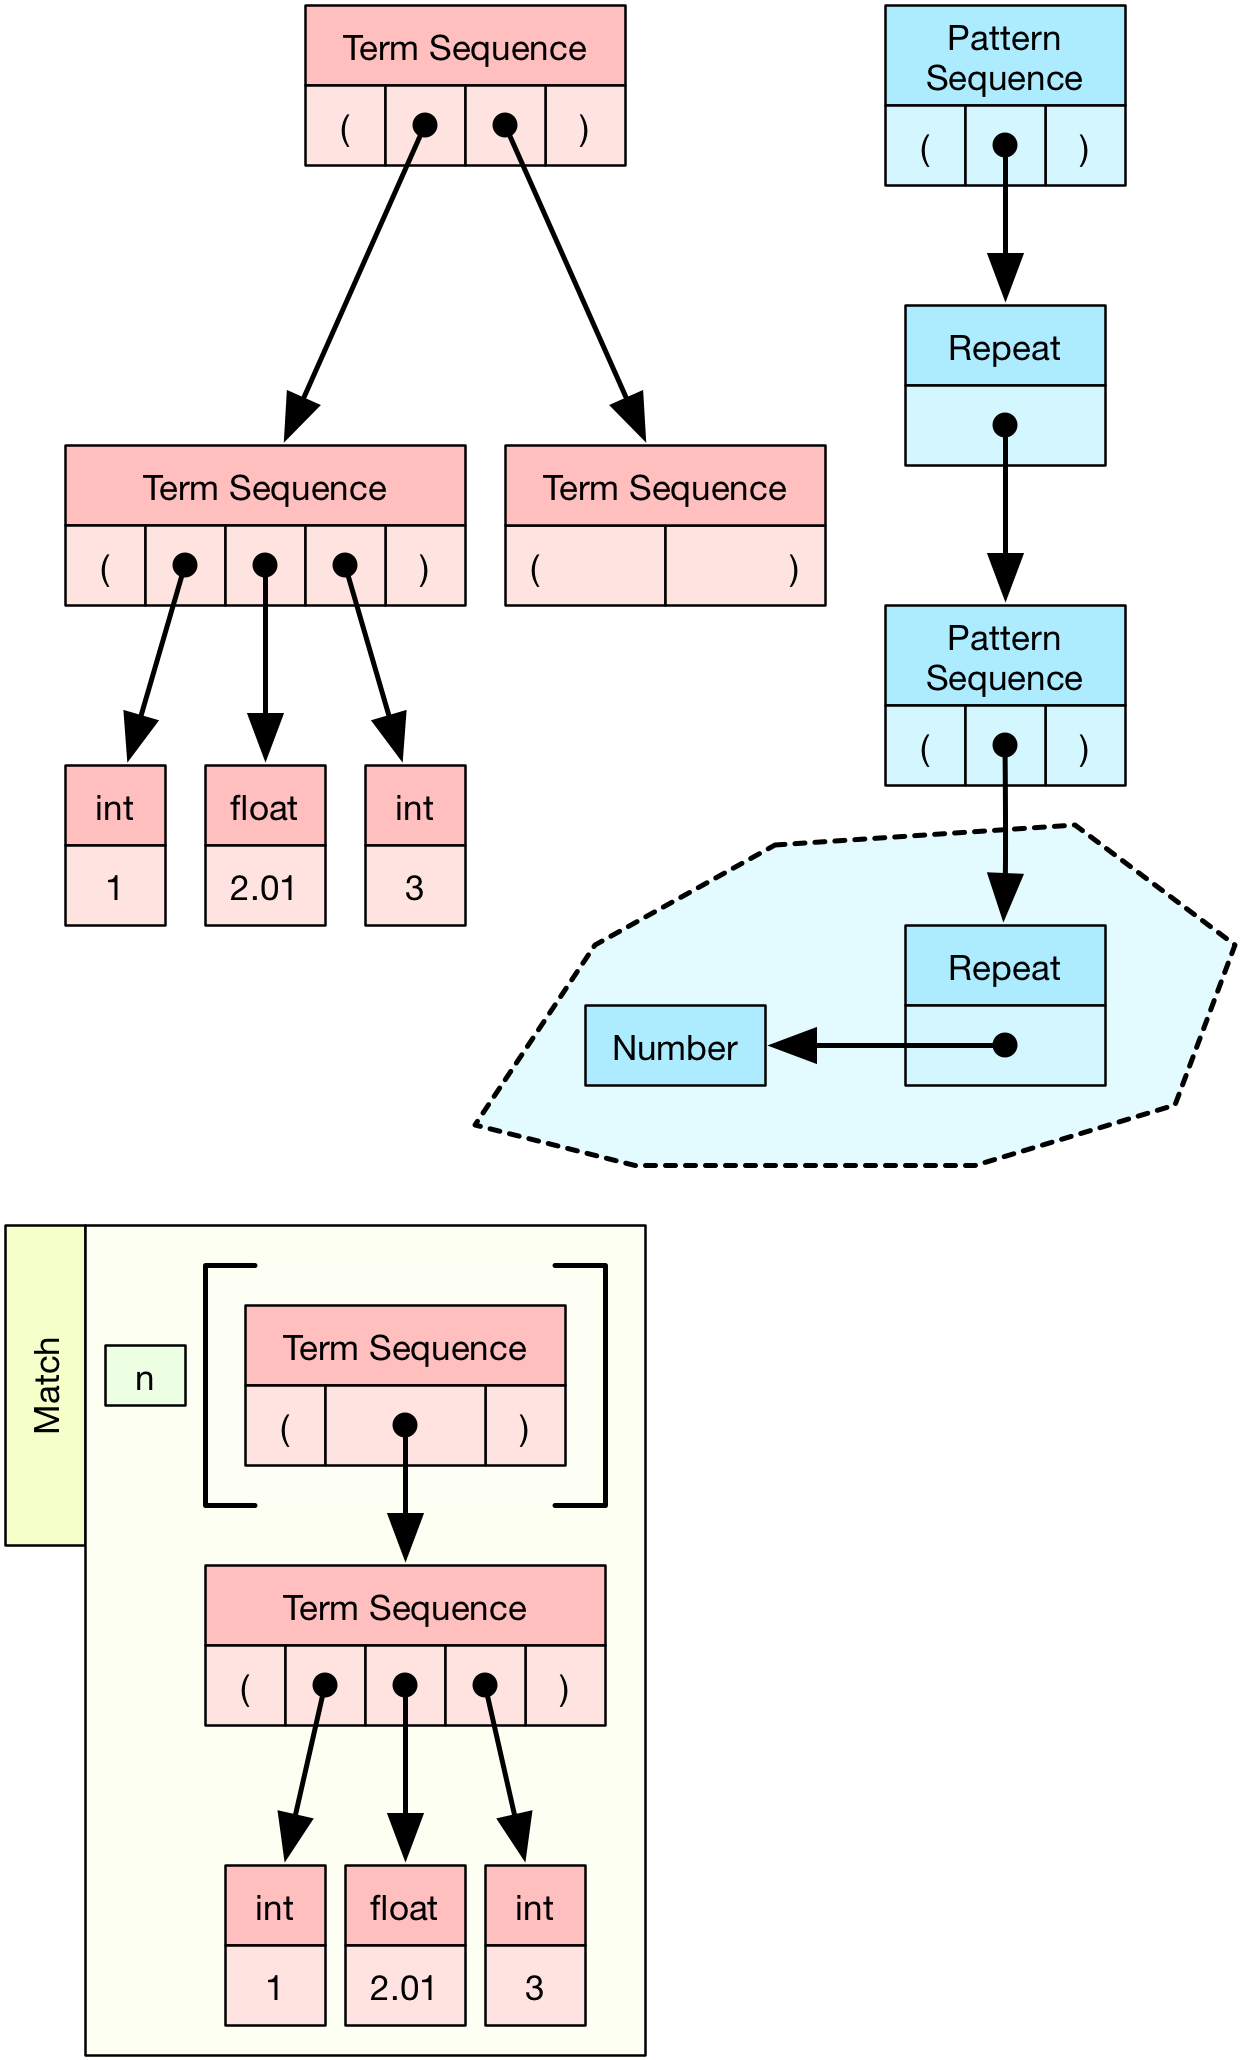
\includegraphics[scale=0.152]{ellipsis-example-fig-g.png}
	\caption{\texttt{decreasedepth("n")} and leave inner ellipsis.}
	\label{ellipsis-example-fig-g}
\end{subfigure}
\begin{subfigure}{0.5\linewidth}
	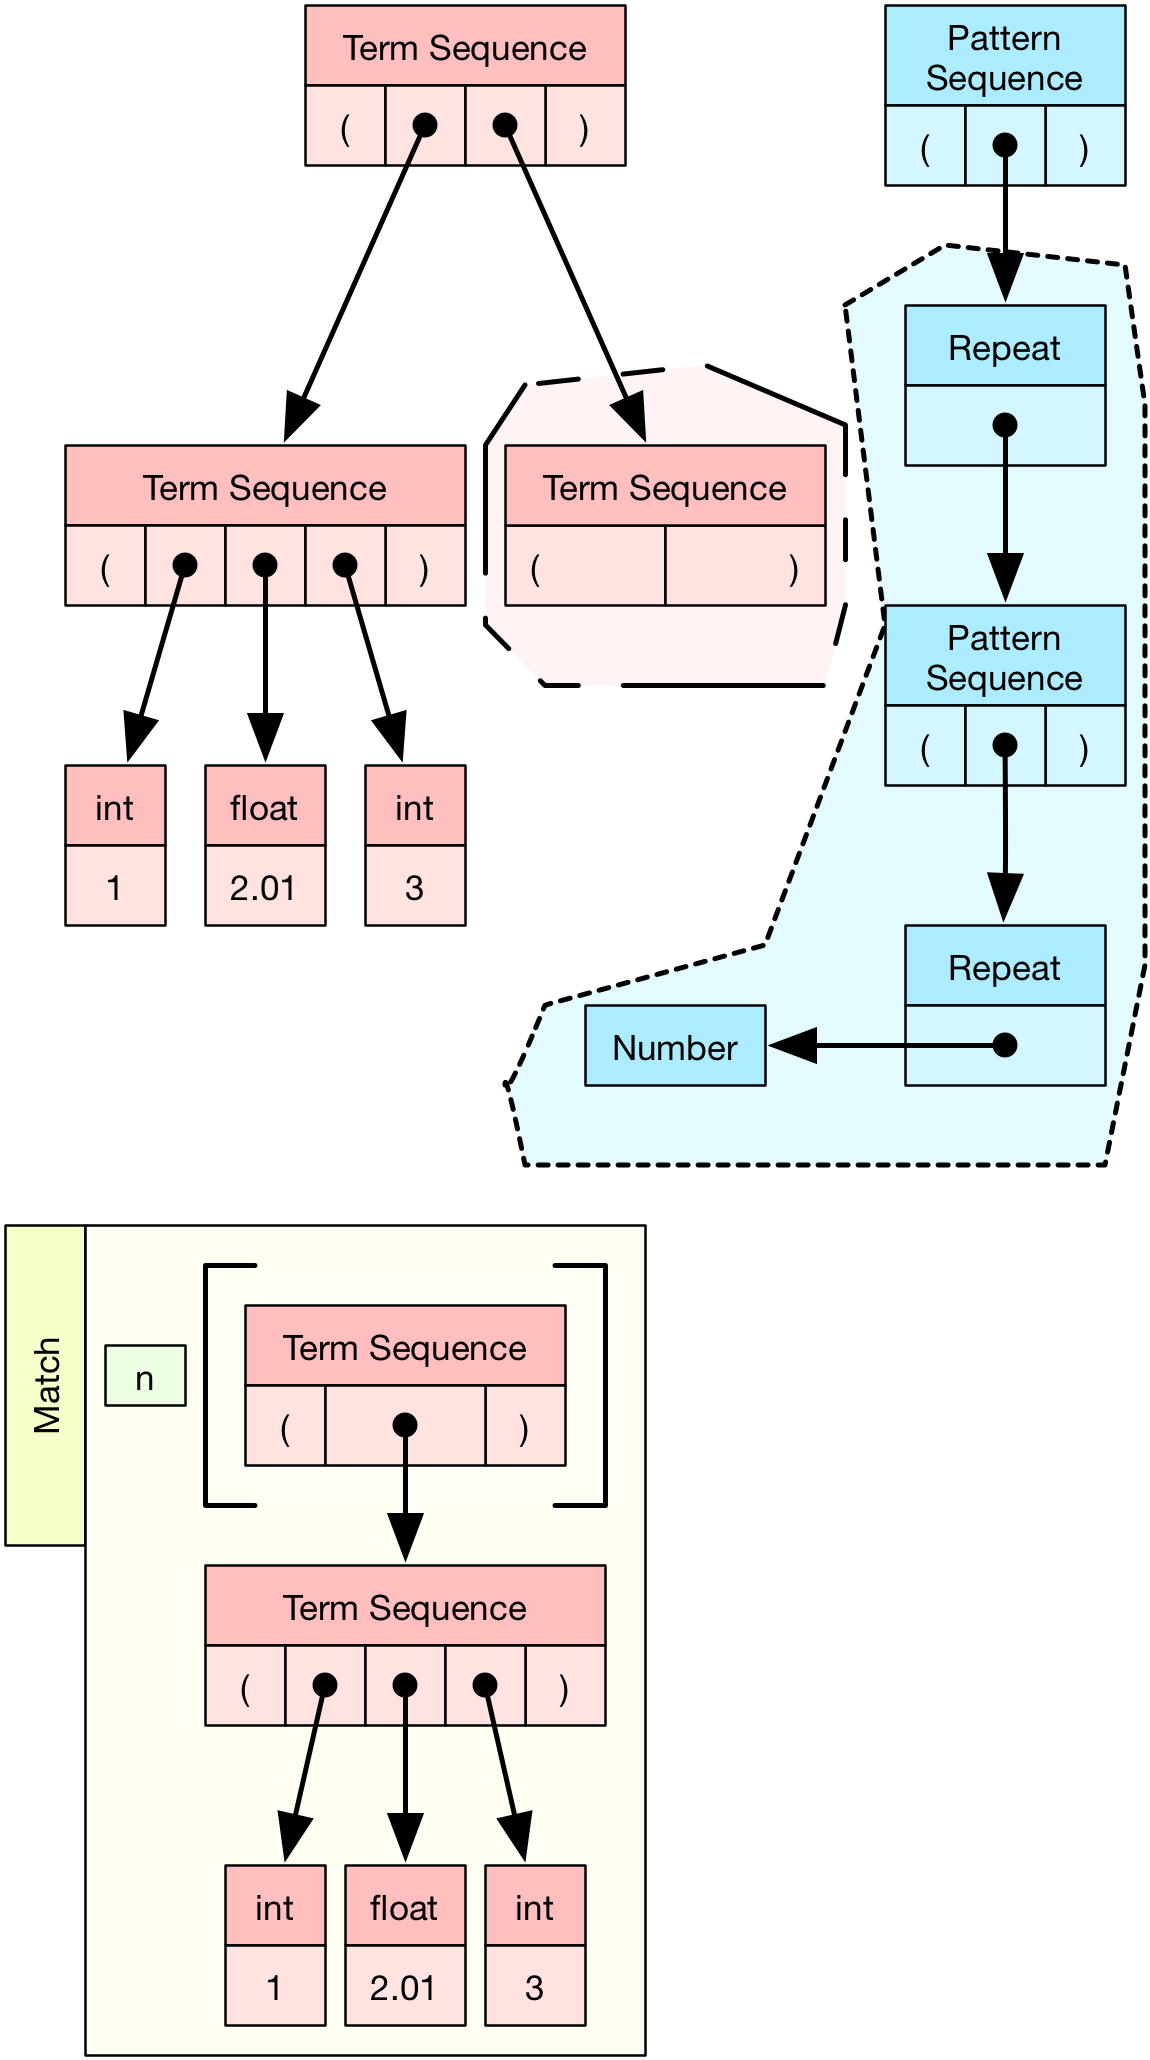
\includegraphics[scale=0.152]{ellipsis-example-fig-h.png}
	\caption{Start processing the next term in the sequence.}
	\label{ellipsis-example-fig-h}
\end{subfigure}
}
\end{figure}
\begin{figure}[H]\ContinuedFloat
\fbox{
	\begin{subfigure}{0.5\linewidth}
		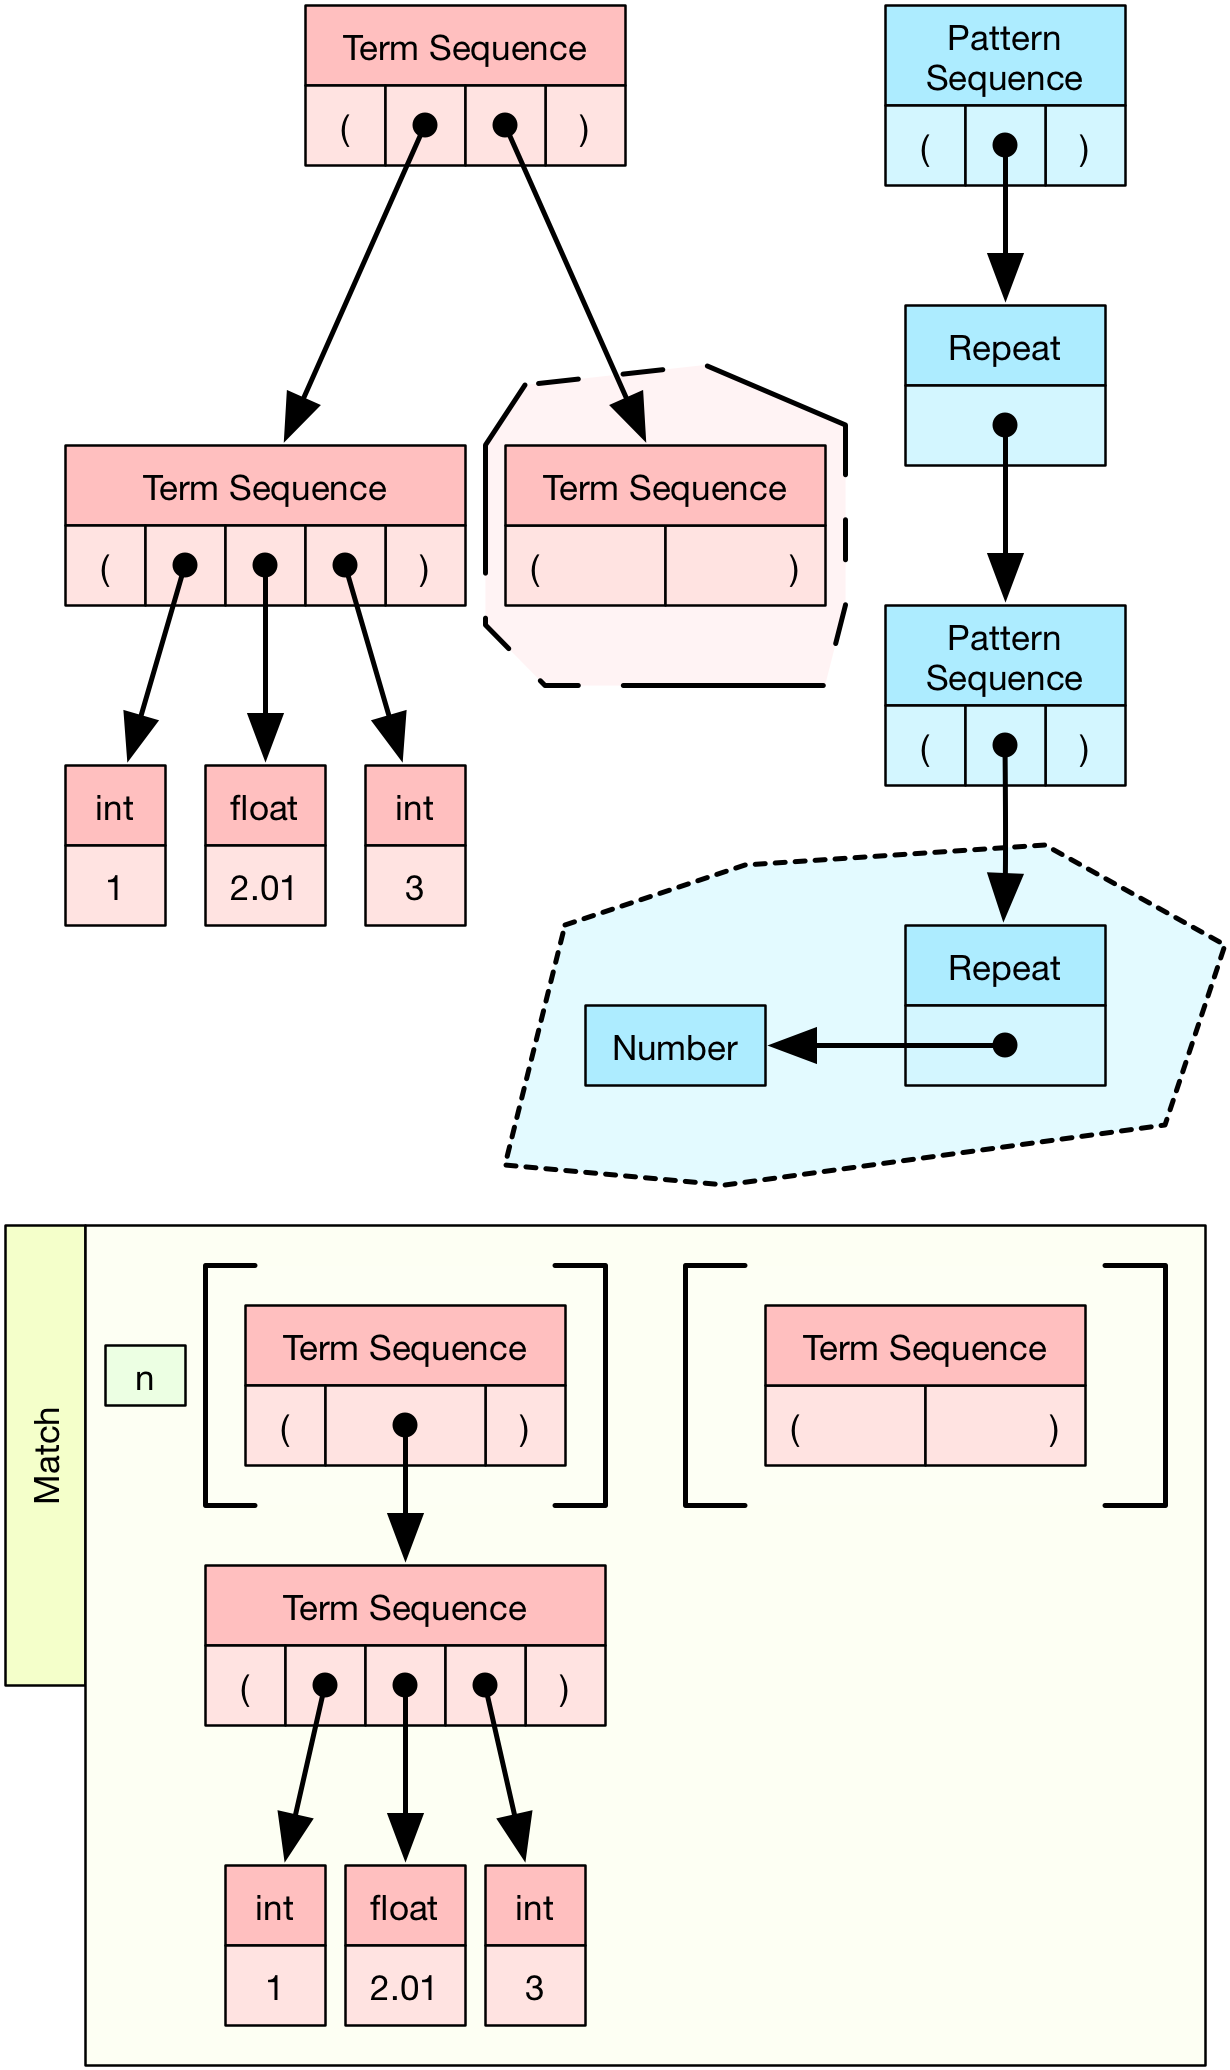
\includegraphics[scale=0.152]{ellipsis-example-fig-i.png}
		\caption{\texttt{increasedepth("n")} after entering inner ellipsis.}
		\label{ellipsis-example-fig-i}
	\end{subfigure}
	\begin{subfigure}{0.5\linewidth}
		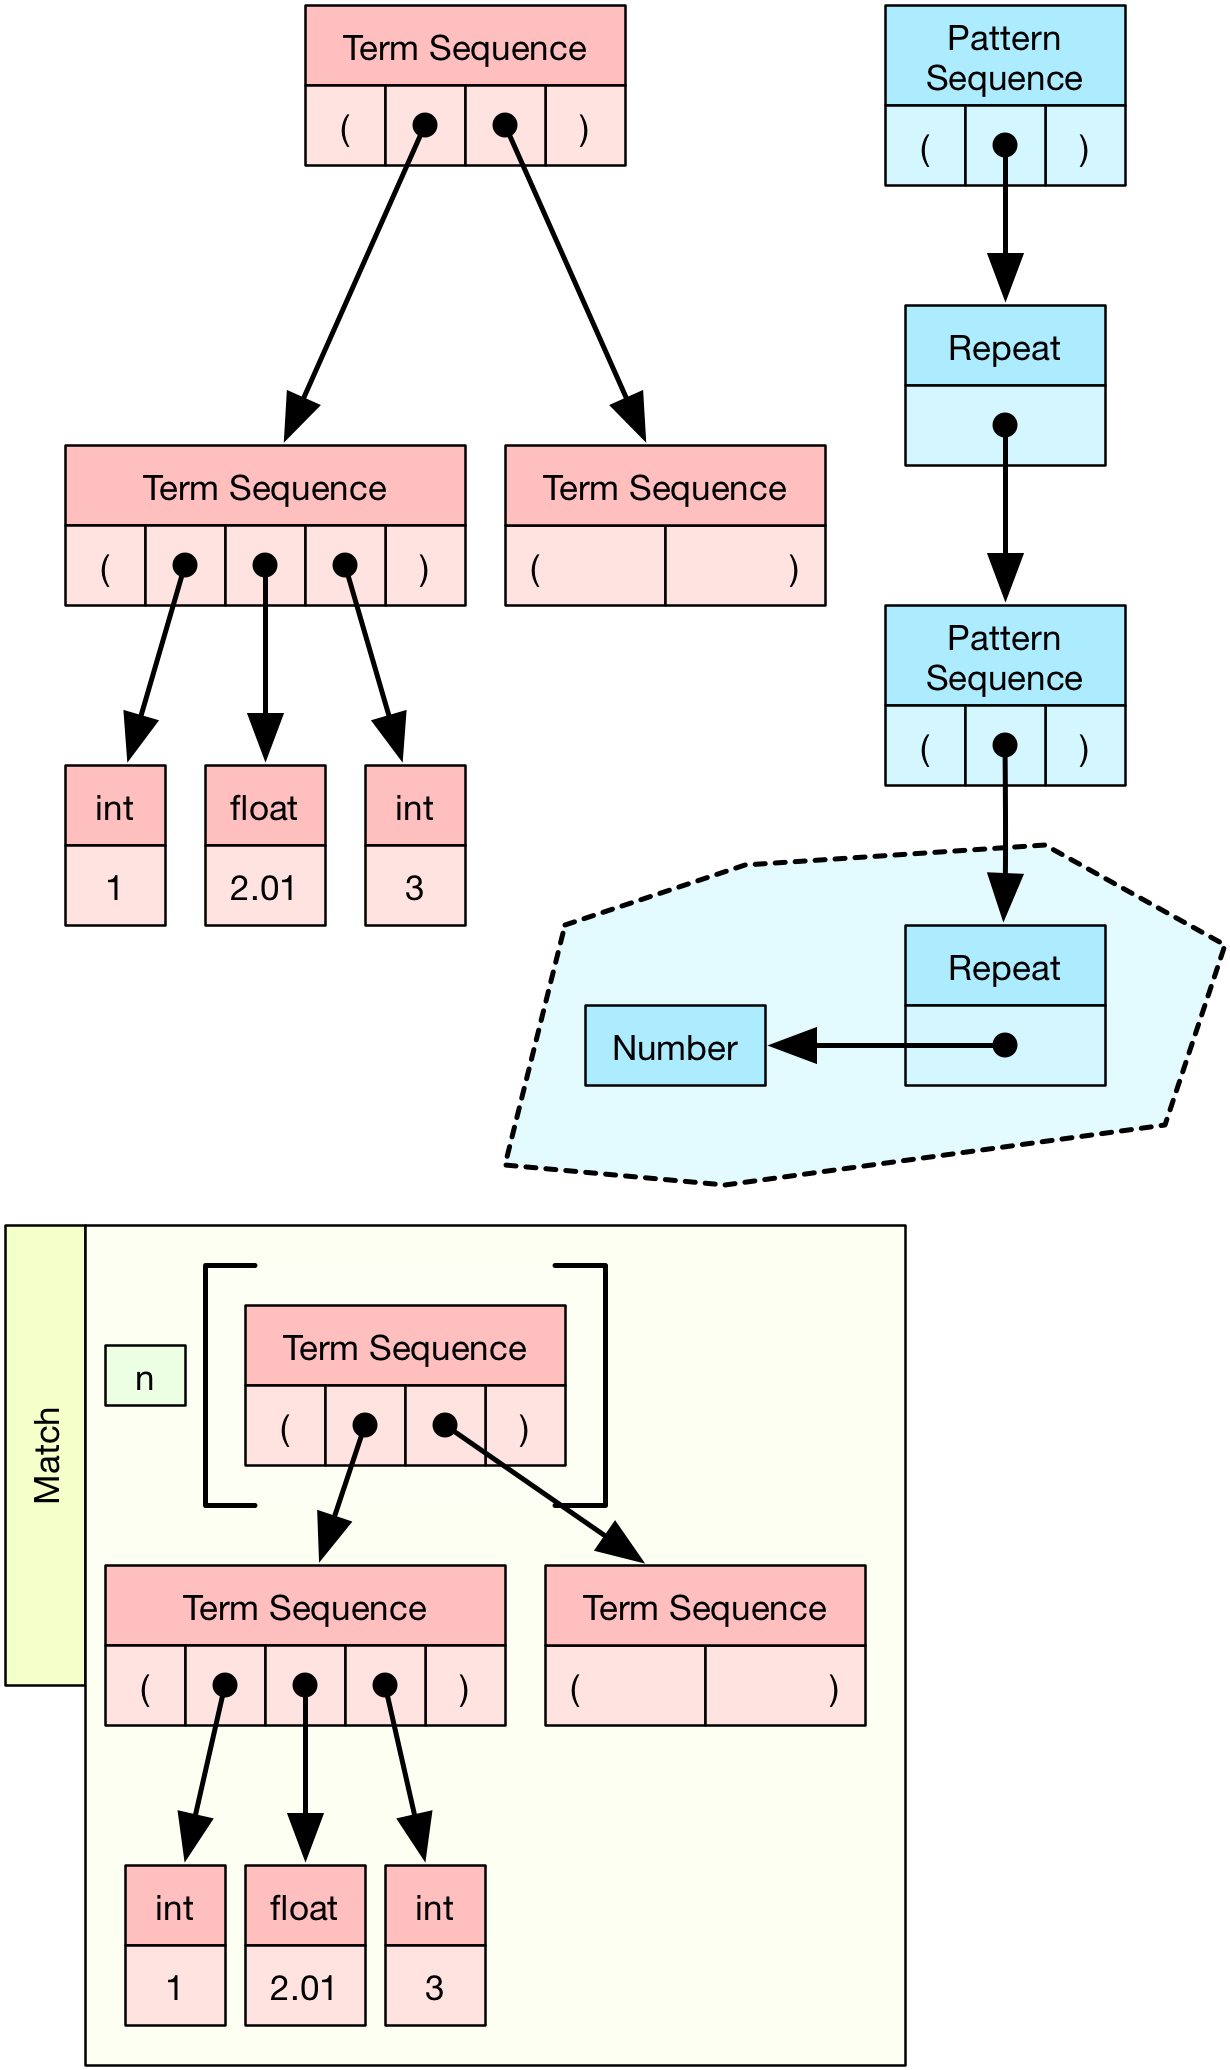
\includegraphics[scale=0.152]{ellipsis-example-fig-j.png}
		\caption{\texttt{decreasedepth("n")} and leave inner ellipsis.}
		\label{ellipsis-example-fig-j}
	\end{subfigure}
}

\fbox{
	\begin{subfigure}{0.5\linewidth}
		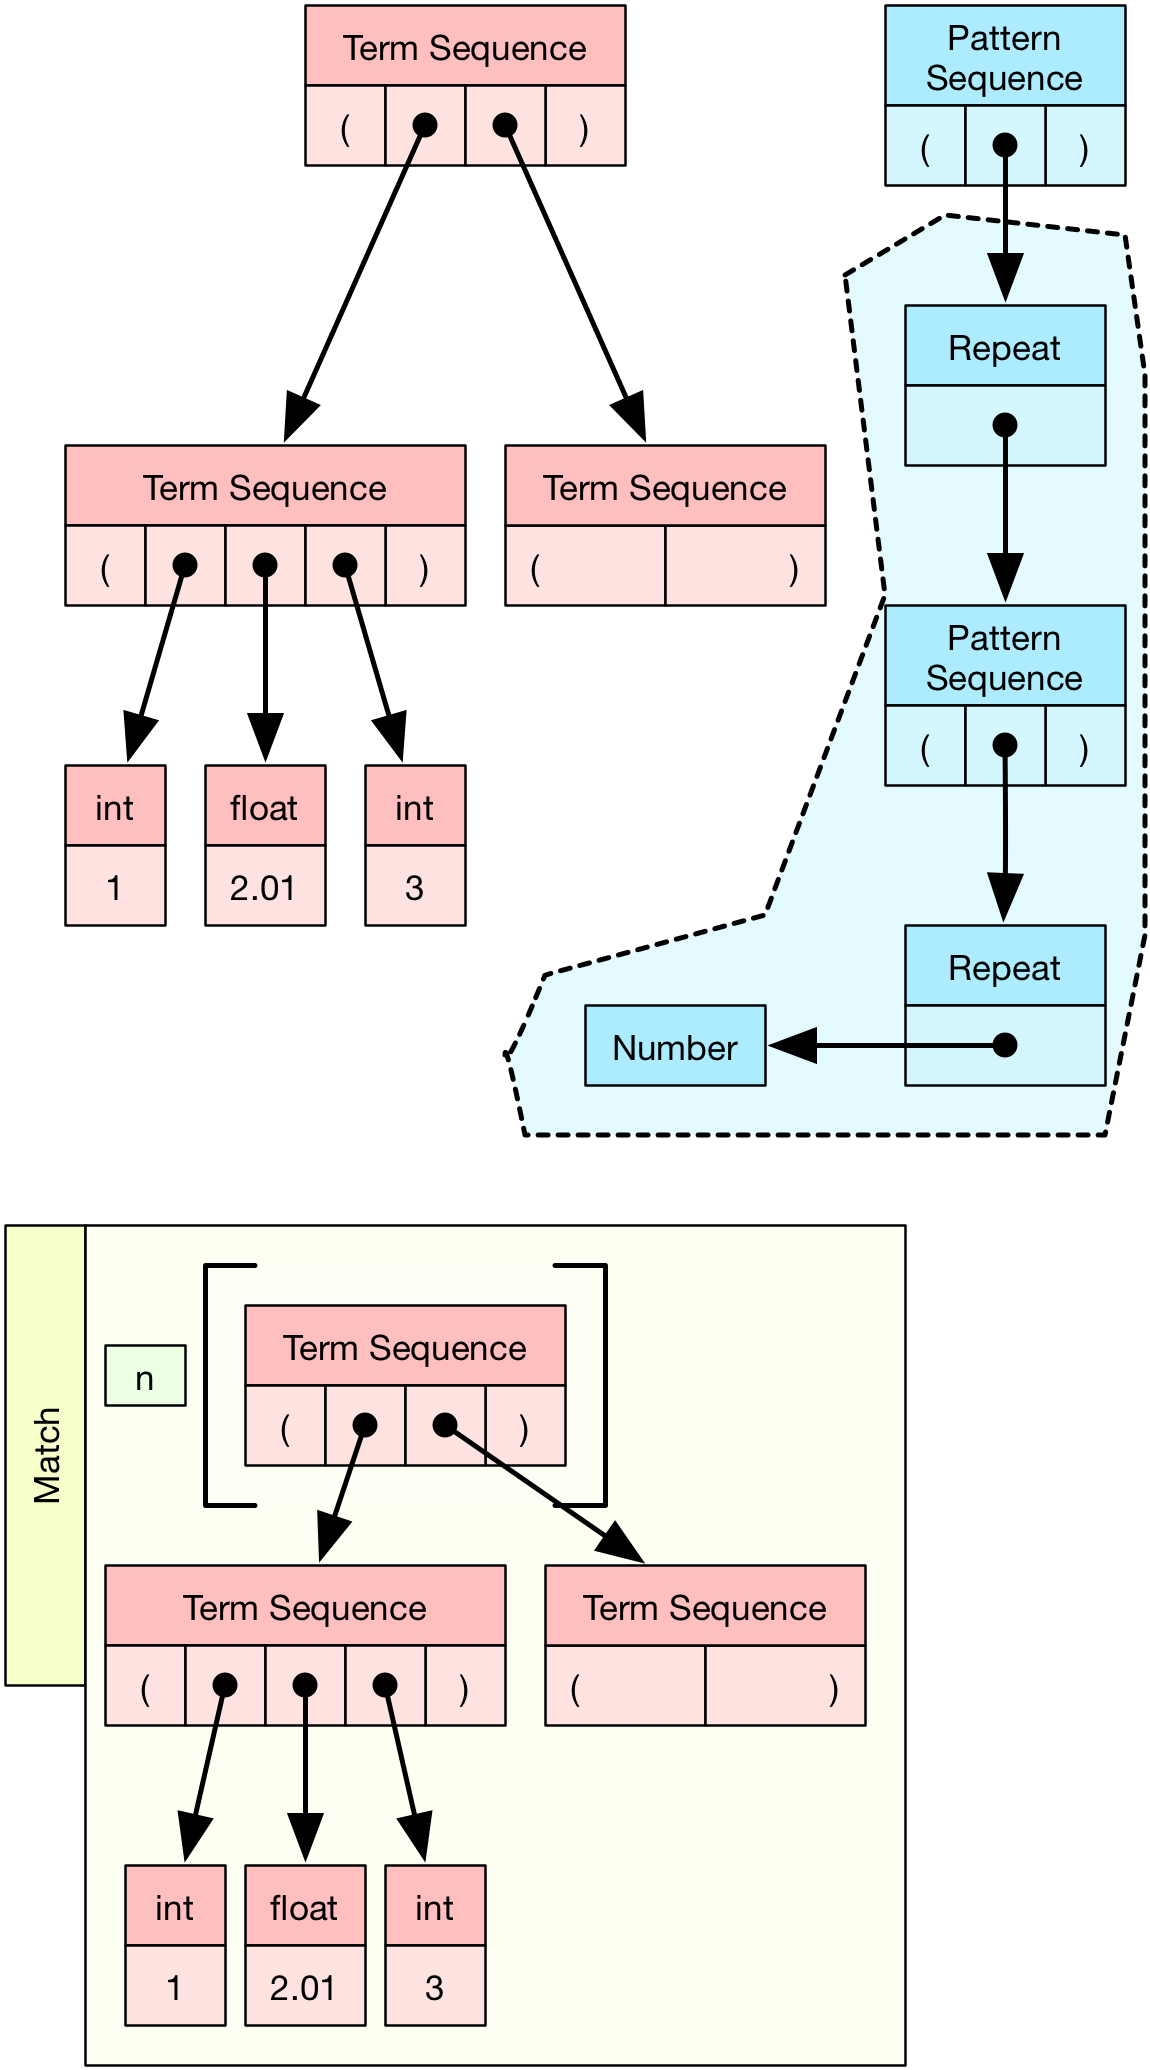
\includegraphics[scale=0.152]{ellipsis-example-fig-k.png}
		\caption{\texttt{decreasedepth("n") and leave outer ellipsis}.}
		\label{ellipsis-example-fig-k}
	\end{subfigure}
}

\end{figure}

One may notice that this example doesn't cover non-determinism when matching patterns under ellipsis. When matching term \texttt{(1 2 3)} against pattern \texttt{n ...} (as shown in Figures \ref{ellipsis-example-fig-d}, \ref{ellipsis-example-fig-e}, \ref{ellipsis-example-fig-f}), the matches shown in Figure \ref{ellipsis-example-matches-1} are returned. To obtain these matches, \texttt{(n ...)} pattern has to be "entered" first, thus setting values of \texttt{head} and \texttt{tail} to zero and the length of \texttt{Sequence}, respectively.Then, pattern \texttt{n ...} is matched in the way explained above (i.e. \texttt{increasedepth}, match pattern \texttt{n}, \texttt{decreasedepth}), resulting in matches in Figure \ref{ellipsis-example-matches-1}.  Now, when exiting function for pattern \texttt{(n ...)}, the only acceptable match among four is the one whose \texttt{head=tail}.

After matching pattern \texttt{(n ...)}, the control flow (see callgraph in Figure \ref{ellipsis-example-callgraph} returns to the function that matches pattern \texttt{(n ...) ...}, and the only returned match is added to the queue. Queue at this point contains a single match. This match is dequeued, and the function for pattern \texttt{(n ...) is called} with term \texttt{()}. \texttt{head} and \text{tail} are set to zero and function for pattern \texttt{n ...} is called. \texttt{increasedepth} is called. Since term \texttt{()} contains no numbers, the only possible match returned by this function is shown in Figure \ref{ellipsis-example-matches-2}.

Finally, the \textit{outer} ellipsis produces matches shown in Figure \ref{ellipsis-example-matches-3} When returning from the function for pattern \texttt{((n ...) ...)}, two of the matches are discarded because \texttt{head != tail}.

\begin{figure}[!htb]
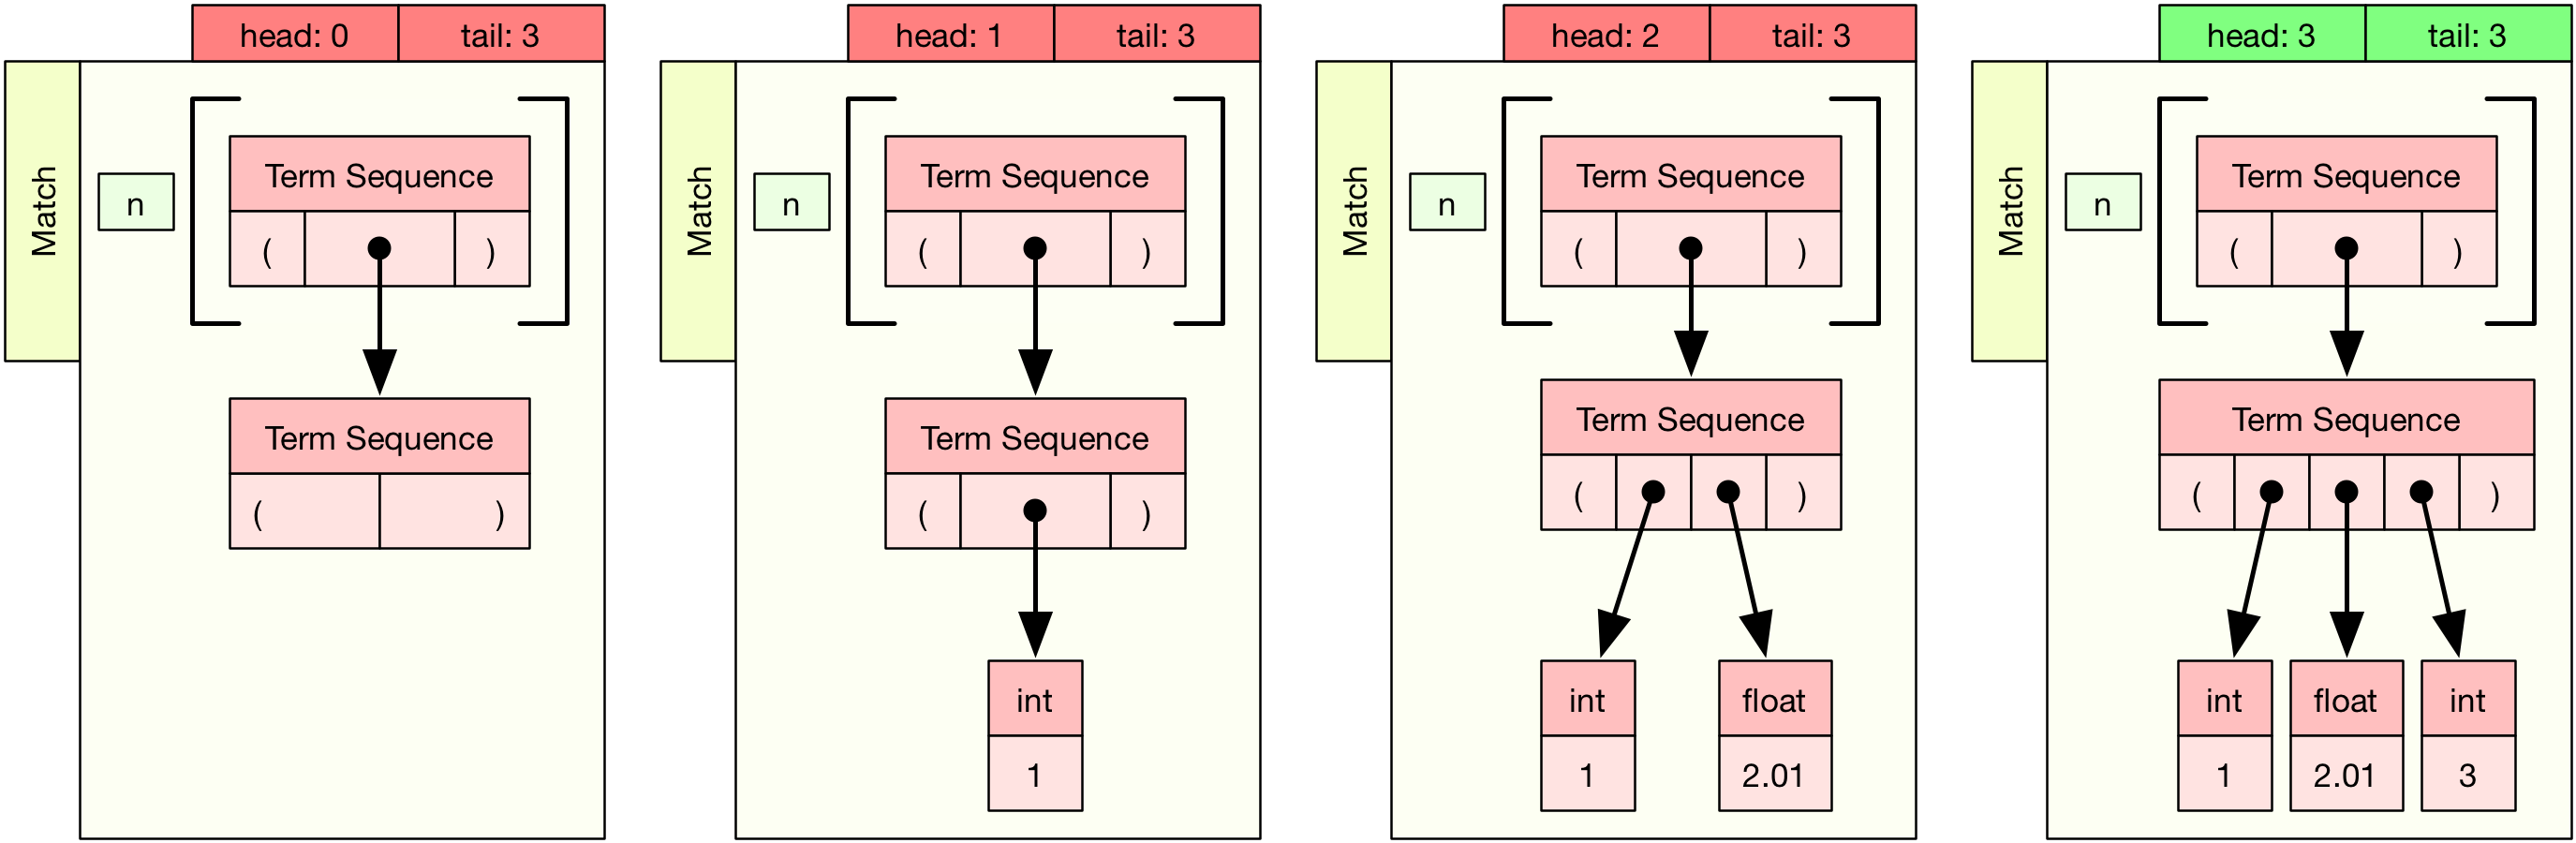
\includegraphics[scale=0.152]{ellipsis-example-matches-1.png}
\caption{Matches returned after matching term \texttt{(1 2 3)} against pattern \texttt{n ...}}
\label{ellipsis-example-matches-1}
\end{figure}

\begin{figure}[!tbh]
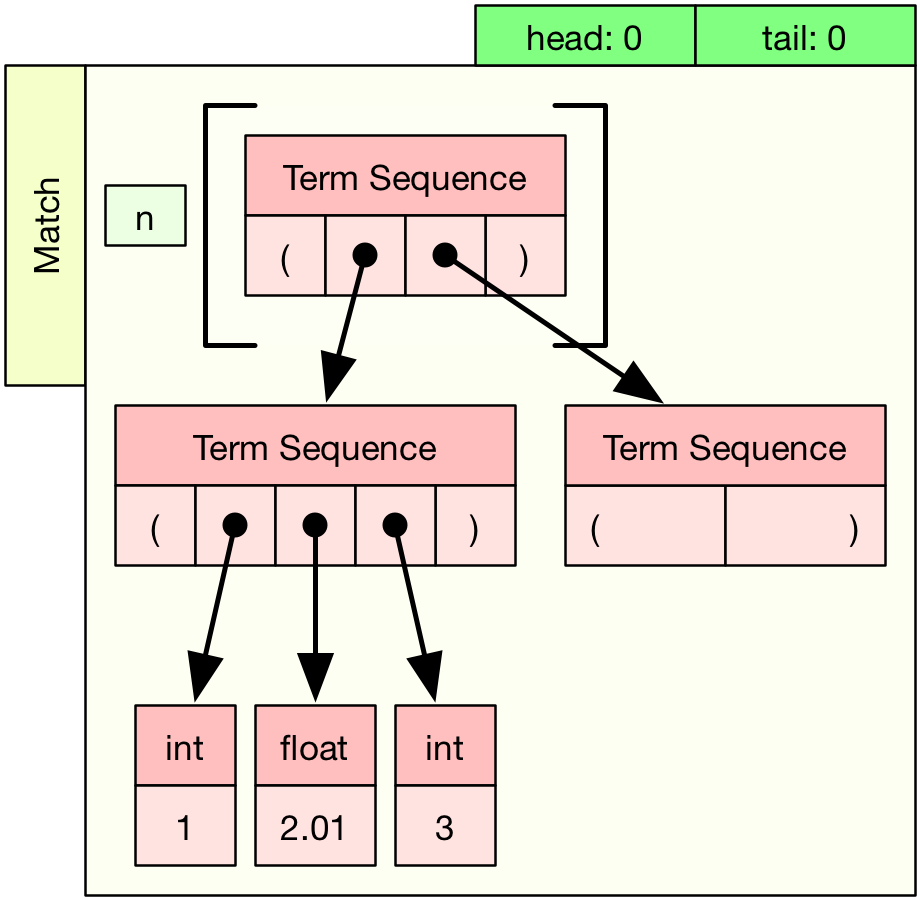
\includegraphics[scale=0.152]{ellipsis-example-matches-2.png}
\caption{Matches returned after matching term \texttt{()} against pattern \texttt{n ...}}
\label{ellipsis-example-matches-2}
\end{figure}

\begin{figure}[!htb]
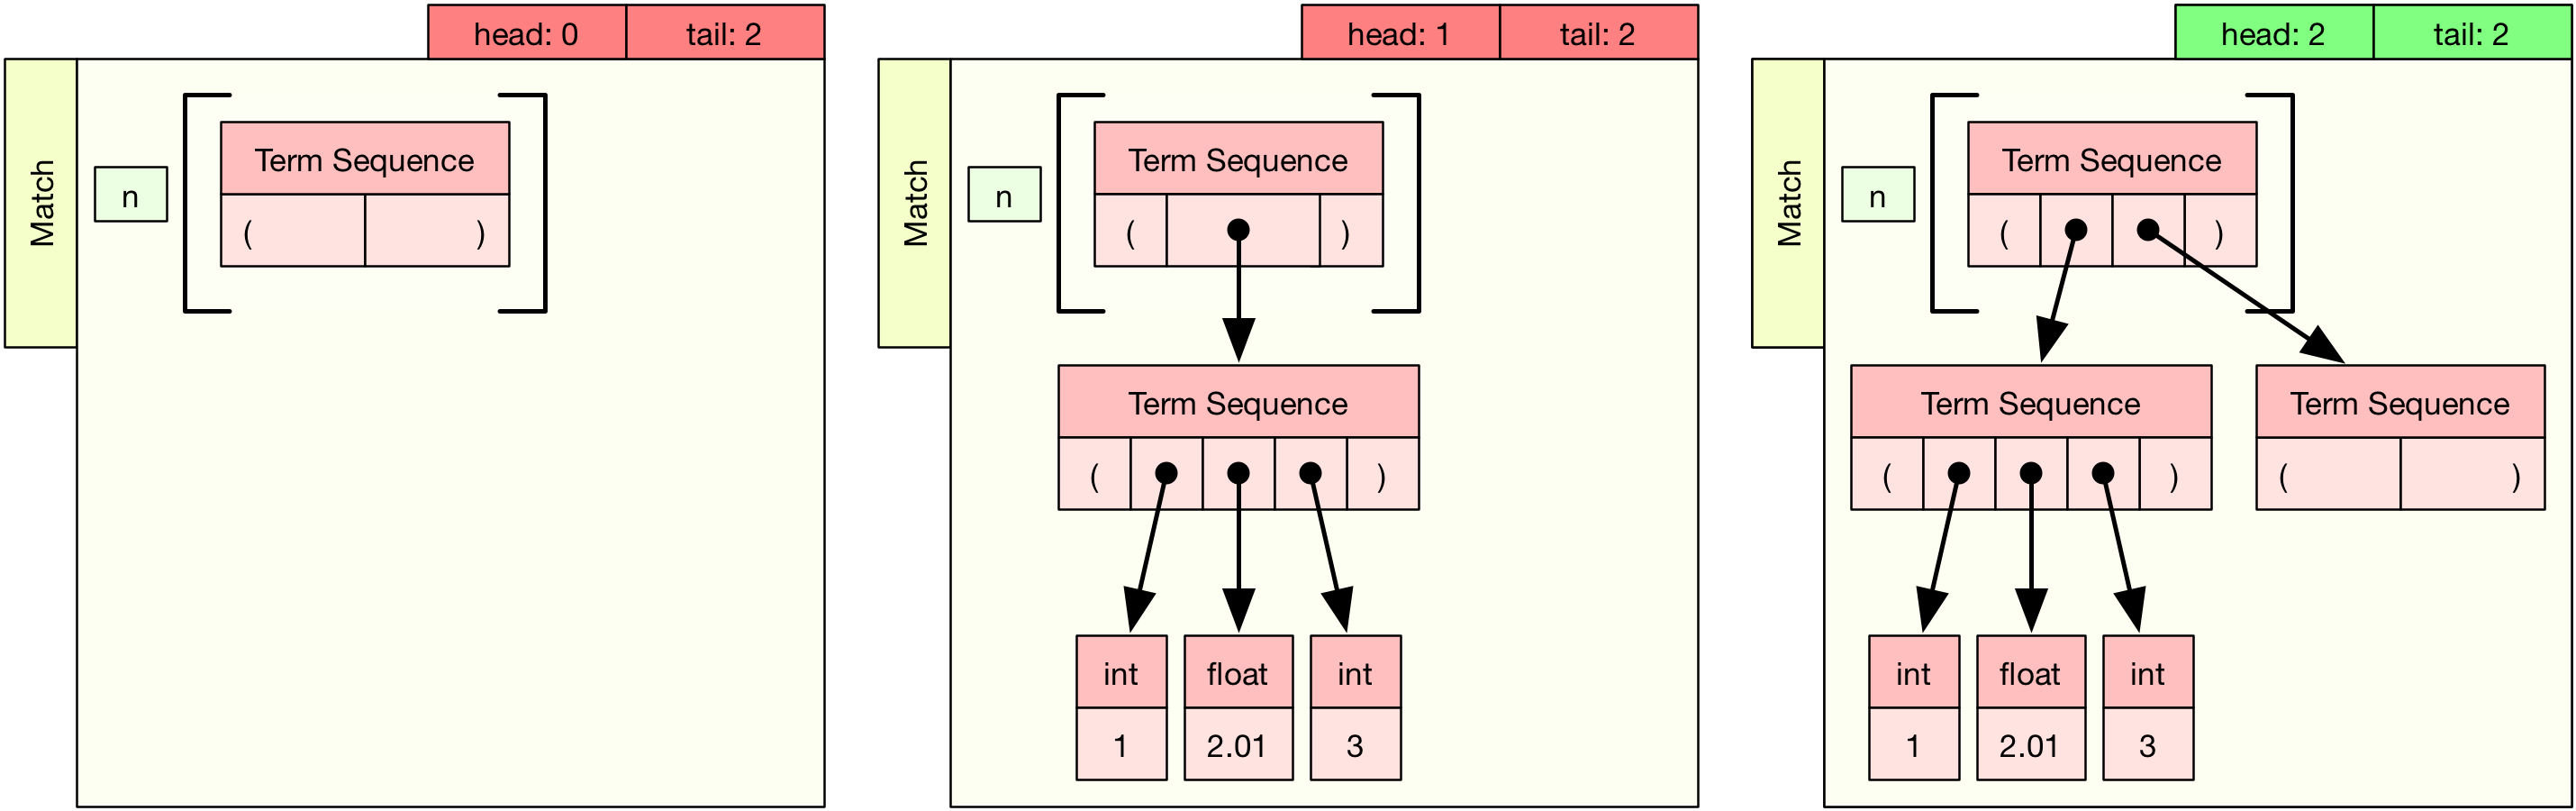
\includegraphics[scale=0.152]{ellipsis-example-matches-3.png}
\caption{Matches returned after matching term \texttt{((1 2 3)())} against pattern \texttt{(n ...) ...} }
\label{ellipsis-example-matches-3}
\end{figure}

